\documentclass[12pt]{article}
%\usepackage[active]{srcltx} to use forward search
\usepackage[ansinew]{inputenc}
\usepackage[pdftex]{graphicx}
\usepackage{picins}%fuer textumflossene Bilder

%/media/daten/home/peter/tut/tex/Latex
%/media/daten/home/peter/text/old/studium/epraktikum/my5/elektronik5.tex
%/media/daten/home/peter/zaurus/sd128/ebbeflut/doc/readme.tex

%now you can jump directly to a special chapter:
\usepackage{hyperref}

\setlength{\oddsidemargin}{1.4cm} %links
\setlength{\evensidemargin}{0.1cm} %rechts

\begin{document}
\addtocounter{footnote}{2}
\pagestyle{empty}
%---------------------------title page-----------------------------------------
\title{ \bf \LARGE The Developer Guide For \\[1cm] genvlin\\[1cm] Documentversion: 1\\TODO: Some things are not reviewed!!}
\author{Peter Karich \footnote{created with \LaTeX{}.}}
\date{Bayreuth, the \today}
\maketitle
\newpage
\setcounter{tocdepth}{2}
\tableofcontents
\newpage
%------------------------------------------------------------------------------
\pagestyle{headings}


\section{Rules}
ALWAYS BE SURE you do not harm the following rules:
\begin{enumerate}
\item Users are stupid! (me too) So test/design the program carefully!
\item \label{2} Performance is important if rule no. 1 wont be harmed!
\item Undocumented methods are not useful for other programmers!
\item Untested code is {\bf not} stable! So write tests (junit)!
\item Avoid machine dependend code!
\end{enumerate}
Actually I violate rule no. \ref{2}, but you can help me!
\section{Open Questions}
Here you are a list of very important todo tasks. Additionally see the todo.txt file - a list available on genvlins webpage (Developer Zone).
\subsection{Solve The Serialization Problems In TopComponent}
I don't really understand ... :-(\\
read/writeExternal and writeReplace/readResolve and write/writeObject?? See Serializable and Externalizable for more information!\\
And how to add the serialVersionID to every class! It should be automatically! Does anybody has some scripts?\\
I know a script (addSerialVer.pl) from the netbeans-feedreader example!
And I know the project from sourceforge! But how do they work?\\
\subsection{Solve The Plot Into Problem!}
Each time the user presses on a "plot-menuitem" (e.g. JFreeChart$\rightarrow$XYLineChart) the action should be stored as "defaultplot-menuitem" so the user can faster plot. The default plot should {\bf add} the XYVector
to the "default-plotpanel" and activate this panel (no new panel!!).\\
{\bf Do you have an idea??}\\
May be there has to be some major changes to the Plugin/PluginPool/Platform interface.
\subsection{Find A Better Solution!}
\label{pluginOQ}
I don't know if you like the PluginPool.get*Plugin(). etc things. They are essential to genvlin!
But this mechanism is not quite nice! So if you have a better idea - let me know!\\
Actually there are two ways to do the same: e.g. for Platform you can do:\\
\begin{verbatim}
PluginPool.getDefault().getPlatform().showPanel(panel,"east");
OR (to be implemented):
PluginPool.getDefault().sendRequest(new RequestEvent() {
  public String getActionContextReason() {
        Platform.SHOW_PANEL;
  }
  public Object getObject() {
        return panel;
  }
  public Object getSource() {
        return this;
  }
});
\end{verbatim}
I prefer the second version, although it looks a bit too complicated and may be: it is slower!\\
But then: we don't need to define an Platform-interface. And there could be more then one plugin listening to that special request!\\
So, which version do you prefer??? Do you have a better idea?\\ \\
Actually there are some hacks around plugin {\bf initilisation}, but they will be removed if we implement a "plugin-registration/init-from-xml" mechanism. Then we can provide a default plugin (for plot/script/...): The user easily change the order of some plotplugins and the first one will be the default!
\subsection{Open Questions In de.genvlin.core.data.*}
\begin{enumerate}
\item Should AbstractCollection provide
\begin{itemize}
\item an own Iterator implementation, so that XYVector.iterator is better?
\item allow concurrentmodification or not?
\item "Number or Object get(int)", "Object or boolean remove(int)"    
\end{itemize}
\item Should there be an InfoVector or not? Which
\begin{itemize}
\item stores or is an AbstractVector (implements Vector $\rightarrow$ new interface?)
\item stores the GUI-width, its plotpanels (or this work via MainPool.get()?)
\end{itemize}
\item Should we allow a one vector twice (or more) in one table or plotpool?? $\rightarrow$ "doubles".
\item Should XYVector get a range wrapper (or index "selecting mechanism") on each AbstractVector, because one could plot via selection and then we don't need all values! but this is not performant!!! may be a hide mechanism is better...   (JFreechart offers an IntervalXYDataSet!!)
\item How would you assume is a math-function like? It is not discrete! But we have to plot and autoscale! So we need a XYInterface-like "discrete" \footnote{I mean the class has its .size, minX, etc methods.} Interface! Hmh I simply extend the XYInterface, but now we have methods like .clear and .remove which makes no sense in a Function class! {\bf So do we need a separation into read- and writeable Collections?}
\end{enumerate}
\section{Requirements Of de.genvlin.core.data.*}
To comply the use cases of genvlin, there are special requirements on the classes in package de.genvlin.core.data.*:
\subsection{All Things Should Have An ID}
they are all iddata. And all will created in MainPool: vector's, xyvector's, pools (except mainpool itself).
\subsection{VectorInterface Requirements}
\begin{enumerate}
 \item "get(Number)"
 \item "set(Number)"
 \item "clear()"
 \item "size()"
 \item "iterator()"? - really necessary?
\end{enumerate} 
\subsection{XYInterface Requirements}
\label{xyvector}
\begin{enumerate}
 \item "Number getX(int)" and Y
 \item "getMinSize()" == "size()"?
 \item getMinX,getMinY,getMaxX,getMaxY
 \item REMOVED: "add(Number x, Number y)", because of Function, see source for details.
\end{enumerate}
\subsection{Pool Requirements}
\label{pool req}there are three types: the mainpool, tablepool and plotpool
\begin{enumerate}
\item{the mainpool should}
	\begin{enumerate}
	\item hold references to ALL vectors (see \ref{pool req}) in the program.
    	\item \label{create new vector}factoryclass for xyvector and vectorinterface implementations and for the pool's (all are iddata).
	\item \label{import} be able to import existing mainpools (from other users/program/..)
    	\item create vectorinterface-implementations via \ref{create new vector}
    	\item create Pool-implementations via \ref{create new vector}
    	\item create xyinterface-implementations via \ref{create new vector}
	\end{enumerate}
\item{the tablepool should (call it VectorPool)}
\label{tablepool}
	\begin{enumerate}
	\item hold references on some vectors. We need xyinterface creation of mainpool!
    	\item create new vectors via \ref{create new vector}
    	\item be created via \ref{create new vector}
    	\item be able to add existing vectors. (This is different to importing! See section \ref{import})
	\end{enumerate}	
\item{the plotpool should (call it XYPool)}
	\begin{enumerate}
	\item be created via \ref{create new vector}
    	\item hold references to xyinterface's (see \ref{xyvector})
    	\item create xyinterface-implementations via \ref{create new vector}
    	\item be able to add other xyinterface-implementation resp. two vectorinterface-implementations.
	\end{enumerate}	
\end{enumerate}
\subsection{DoubleVector Requirements}
should be a performant implementation of vectorinterface (Question: Is the do we need a DoubleVectorInterface?)
\subsection{UML Diagram}
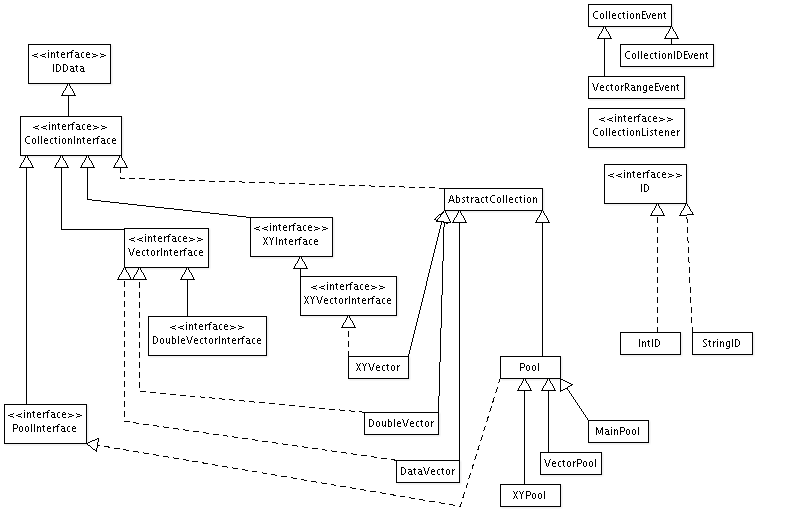
\includegraphics[width=\textwidth]{uml.png}\\%parpic
\section{Module Dependency Graphic}
He you are a roughly overview of the genvlin-suite:\\[1cm]
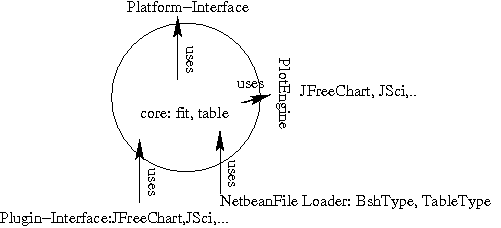
\includegraphics[width=\textwidth]{dependencies.png}\\%parpic
There should be no dependencies between the plugins! So we have to define an interface like:
PluginPool.getScriptInterpreter and PluginPool.getDefaultPlotEngine and PluginPool.getMathEngine\\
But how do the special engine-interface's look like? May be it is easier to {\bf have} dependencies between the plugins ... ??
\section{Currently Used Plugin Mechanism In genlinv}
I need your comments on Openquestion in section \ref{pluginOQ}!!
\begin{verbatim}
\end{verbatim}
\section{Singletons In genvlin}
\begin{itemize}
\item MainPool.getDefault
\item GProperties.getDefault
\item PluginPool.getDefault
\end{itemize}
\section{Some Netbeans Explantations}
May be this is only useful for newbies (e.g. me) to netbeans.\\
If you add a new plugin (plotplugin): create a moduleinstaller via right clicking folder.\\
AND you have to substitute the first line with:\\
\#is.autoload = true in project.properties file.\\
and then clean and build the whole project! Or:\\
Right click$\rightarrow$ properties $\rightarrow$ API Versioning $\rightarrow$ Regular instead of AutoLoad!
{\bf Hint:} Use the same "Regular" procedure to add a new filesystem!
\subsection{Netbeans Calls}
\begin{enumerate}
   \item{dataloader constructor}
    This will hapen whil module loading: dataloader.initialize().
    initialize() is called only once - the first time a shared is used. 
    Not for each instance!  (dataloader extend from SharedClassObject)
    The call is a result of specifing the loader in the manifest file.
   \item{dataloader findPrimaryFile}
	\begin{enumerate}
	\item ??? if we have to deserialize: this method will be
            called from ModuleManager.enable() $\rightarrow$ initilizeLookup().
   	\item if netbeans wants to initialize the nodes it will also be called.
	\end{enumerate}
   \item dataloader actionsContext
   \item dataloader createMultiObject $\rightarrow$ new TableDataObject
   \item action.gethelpctx() + iconResource() + getName from SystemAction.getValue() called after modules turning on.
   \item deserialization of topcomponent,result: calling TopComponent.readExternal
   \item the favourites main-node construction,	result: calling 2-times(??) "dataloader.findPrimaryFile $\rightarrow$ createMultiObject()	$\rightarrow$ createPrimaryEntry"
   \item tabledataobject.createNodeDelegate: is called only once per dataobject
\end{enumerate}
\subsection{If The User Do Something}
\begin{enumerate}
   \item ImportAction-MainMenu if we click file$\rightarrow$ ImportAction.mode will be called. Further calls see \ref{dataloader}
   \item ImportAction-ContextMenu if we right-click file$\rightarrow$ ImportAction.mode will be called. Further calls see \ref{dataloader}
   \item Open-ContextMenu: ??? TableTopComponent.run from EventQueue
   \item DoubleClick on a table node
	\begin{enumerate}
	\item \label{dataloader}result: calling dataloader.actionsContext() (only once per run!)
	\item PopupSupport.mouseClicked calls
	 \begin{itemize}
           \item ImportAction.cookieClasses + .mode()
           \item .asynchronous
           \item NodeAction.DelegateAction.actionPerformed
                    calls ImportAction.performAction in an ActionRunnable
           \item ImportAction.performAction
		\begin{itemize}
   		\item node.getCookie $\rightarrow$ ImportAction.mode() (2-times?)\\
   		\item Thread.run $\rightarrow$ TableOpenSupport.createcloneable $\rightarrow$ tabletopcomp.CONSTRUCTOR
		\end{itemize}
	\end{itemize}
	\end{enumerate}
   \item expand the main node, result: nb create the nodes $\rightarrow$ for every node it calls dataloader.findPrimaryFile\\
     if mimetype fits nb calls createMultiObject (this invokes createPrimaryEntry)
   \item expand a table node
	\begin{itemize}	
	\item result: TableChildren.addNotify will called $\rightarrow$ TableGUISupport.getTable will be called in a thread $\rightarrow$ import
	\item result: calling TableChildren.createNodes (for n-times) because of calling setKeys()
	\end{itemize}	
\end{enumerate}
\section{My SVN Help}
see subversion at tigris for a better tutorial!
\subsection{Perhaps You Mistakenly Removed A File From Version Control}
in:  svn status README\\
out: README\\
in:  svn status
$\rightarrow$ list all files recursivly which are "(M)odified", "not under vc"(?)
locally deleted(!) and file which will be "(A)dded" added with the next commit.\\
in:  svn delete README\\
out: D         README\\
in: svn revert README\\
out: Reverted 'README'\\
in: svn status README\\
out: README\\
\subsection{See All Commitmessages}
svn log
\subsection{List Content Of A File}
svn cat
\subsection{List All Versioned Files}
svn list --verbose file:///home/peter/quell/genvlin-suiteSVN/
\section{Some Things I Learned And I Don't Want Forget}
\subsection{Netbeans GUI}
See also NbQuestions.txt\\
\begin{itemize}
\item where is our output window? $\rightarrow$ log(ex, TRUE) will not work!\\
Now it works! Include mostly all harnes-cluster plugins ... Why that???\\
may be this is the reason:  
{\bf Problem when deserializing TopComponent for tcID:'output'. Reason: Top component output could not be located or loaded from Components folder. Cannot resolve default platform. Probably either "org.netbeans.modules.apisupport.harness" module is missing or is corrupted.}
\item You have to add the IOProvider token in "right-click module"$\rightarrow$"Properties"$\rightarrow$"Libraries"\\
\item shift esc for maximizing the editor
\item Alt-Shift-o $\rightarrow$ lookup a java class
\item Shift-F4    $\rightarrow$ select from open editor-component, this is same as:
\item Ctrl-Tab    $\rightarrow$ select from open editor-component.
\end{itemize}
\subsection{General Java Things}
\begin{itemize}
\item "AbstractVector.this.someMethod()" could be called from inner classes\\
\item this is a valid java expression ";;;;"\\
\item "static" before an inner "class" provides to use static variables in inner class or use the inner class from static context.
\item Alt-Shift-O for quick java class opening
\item anonymous constructor:
\begin{verbatim}
new Thread() {
    { start(); } //<--- !!
    public void run() { ... }
};
\end{verbatim}
\item generate bytecode via: javap -c
\item Thread t = ...; Runtime.getRuntime().addShutdownHook(t);
\item To avoid the possibility of deadlock, you must take extreme care that Swing components and models are created, modified, and queried only from the event-dispatching thread In that case (ComponentEventDemo), sometimes when you launched the demo, it would not come up because it would deadlock when updating the text area if the text area had not yet been realized, while other times it would come up without incident. Implementations of abstract API objects in these packages (the Filesystems API, Datasystems API, and Java Hierarchy API) should also follow this convention (completely thread-safe) and use language-level synchronization where needed. Such implementations include custom filesystems, data loaders, data objects, cookie supports, hierarchy element implementations, etc. It is also useful to post a request to the processor in the middle of GUI code, if the request might take a perceptible amount of time to complete. $\rightarrow$ use GTask!
\end{itemize}
\section{genvlin Needs Your Help!}
Help is wanted! See the Developer Zone on the homepage! We need:\\
\begin{itemize}
\item java developer
\item web layouter
\item private or industrial sponsors
\item native english speakers to review all the doc and source
\item translators to translate the program and the doc into various languages
\item tester (with and without java knowledge)
\end{itemize}
A developer will be registered (he/she gets svn-write access) if he/she solves two small tasks or one big in the todo-list! (It is also okay if he/she send me his/her own tasks for genvlin and solved that...)
%If there are at least 10 developers I will choose the {\bf "programmer of the year"} and he/she will 
%recieved 50 EUR on his web.de account (registration is free! sorry to paypal users.)
\section{Contact}
\label{contact}
Visit the genvlin web page at: http://genvlin.berlios.de/\\
My email adress: sourcemaker2000-genvlin at yahoo dot de\\
\end{document}
